\chapter{The Compact Muon Solenoid Experiment}
\label{chap:I-3-cms}

	The Compact Muon Solenoid (CMS) \cite{1748-0221-3-08-S08004} is a multi-purpose particle detector recording the collisions provided by the LHC. It was, along with ATLAS, the first experiment officially approved for the LHC by the CERN research board in January 1997 after a long evalution process of the letter of intent published four years earlier by the collaboration. The construction of the detector started in 2005, after the excavation works of the cavern finished, and spanned until 2008. Since then, CMS has been proficiently taking and analyzing data, and announced on July 4th 2012 the discovery of the Brout-Englert-Higgs boson, one of the most significant results of the collaboraton.

  \section{Overview}

    At nominal energy and luminosity, the LHC produces around 20 proton-proton collisions per BX which results in around 1000 particles in the final state. In order to distingish physical processes with great precission CMS has to ensure good identification and reconstruction of the particles. To this end, the detector was built around four requirements:
    \begin{itemize}
      \item Good muon identification and momentum resolution over a wide range of momenta and angles, good dimuon mass resolution ($ \approx $ 1\% at 100 GeV), and the ability to determine unambiguously the charge of muons with p < 1 TeV;
      \item Good charged-particle momentum resolution and reconstruction efficiency in the inner tracker. Efficient triggering and offline tagging of $ \tau $'s and b-jets, requiring pixel detectors close to the interaction region;
      \item Good electromagnetic energy resolution, good diphoton and dielectron mass resolution ($ \approx $ 1\% at 100 GeV), wide geometric coverage, $ \pi^0 $ rejection, and efficient photon and lepton isolation at high luminosities;
      \item Good missing-transverse-energy and dijet-mass resolution, requiring hadron calorimeters with a large hermetic geometric coverage and with fine lateral segmentation. \\
    \end{itemize}

    \begin{figure}[h!]
      \centering
      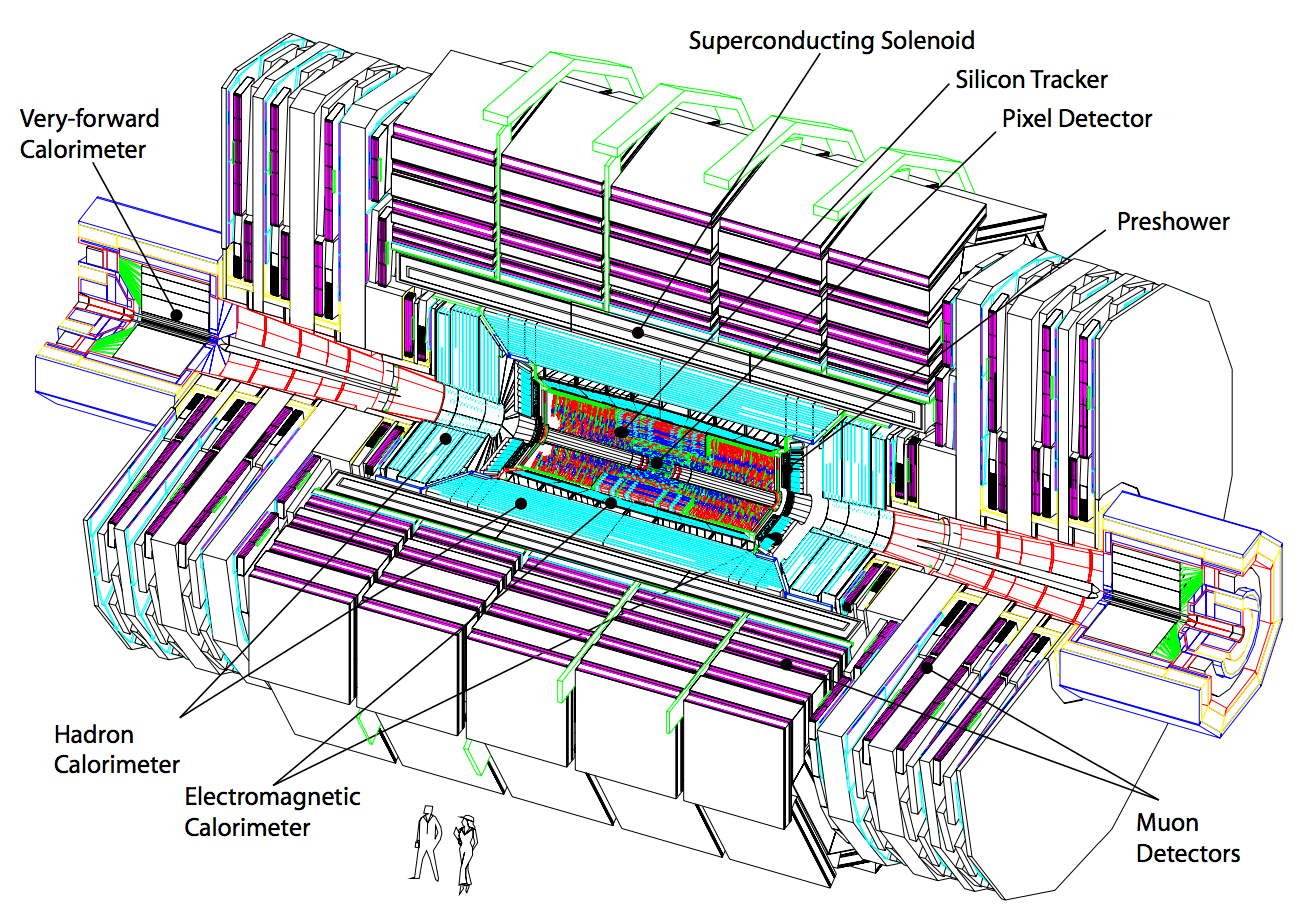
\includegraphics[width=\textwidth]{img/I-3-cms/cms.png}
      \caption{Schematic representation of the Compact Muon Solenoid detector installed at LHC \cite{1748-0221-3-08-S08004}.}
      \label{fig:I-3-cms-global-view}
    \end{figure}

    These requirements are met through the subdivision of CMS in various detection systems each specialised in the reconstruction of a given type of particles. The overall layout of CMS, shown in Figure \ref{fig:I-3-cms-global-view}, is divided into the barrel and the two endcaps, regions where the detectors are respectivly placed in parrallel and perpendicularly to the beam pipe. At the center of the detector, closest to the interaction point, lies the inner tracking system. Composed of 3 layers of silicon pixels and 10 layers of silicon strips detectors, it is designed to detect the passage of any charged particle with high precision. Surrounding the tracking system are the electromagnetic and hadronic calorimeters which respectivly measure the energy of electrons and photons, and hadrons. These detectors are placed inside a superconducting solenoid magnet which produces a strong 3.8 T field that bends charged particles and allows for precise momentum measurments. Outside of the magnet, three different technologies of muon detectors are placed on large iron yokes. Furthest from the interaction point are the very-forward calorimeters which intercept particles with low flighing angle.

    The coordinate system used in CMS has its origin at the nominal interaction point of the beams, the y-axis pointing upwards, the x-axis pointing toward the center of the LHC, and the z-axis directed along the beam direction. The polar coordinates (r, $ \phi $) are defined in the x-y transverse plane and the widely used pseudorapidity $ \eta $ is taken to be
    \begin{equation}
      \eta = - \ln\left( \tan\left( \frac{\theta}{2} \right) \right) ,
    \end{equation}
    where $ \theta $ is the azimuthal angle between the z-axis and the transverse plane.

  \section{The Inner Tracking System}

    The inner tracking system of CMS is designed to provide a precise and efficient hit information on the trajectories of charged particles.  The proximity of the detectors to the beam pipe yields a high particle density of up to 10$^8$ particles per cm$^2$ at a radius of 4 cm. This justifies the need for a high granularity and fast response time to unambigously assign particles to the correct collision. However, these features come with an elevated power comsumption which in turn requires efficient cooling infrastructure. In order to keep the material budget of the tracker as low as possible, a compromise was found to use two technologies: silicon pixels close to the beam pipe to provide a high granularatiy, and silicon strips further away to reduce the material budget. \\

    The layout of the detectors is shown in Figure \ref{fig:I-3-tracker}. The silicon pixels (PIXELS) are installed on three cylindrical layers in the barrel and two disks in each endcap. These detectors cover an area between radii of 4.4 cm and 10.2 cm and a pseudorapidity $|\eta|$ > 2.5. The silicon strips (TIB, TOB, TEC, and TID) occupy a radial region between 20 cm and 116 cm and are divided in different sectors with a total of 10 layers in the barrel and 12 disks in each endcap. The segmentation into sectors corresponds to the various strip geometries and arrangment. \\

    \begin{figure}[h!]
      \centering
      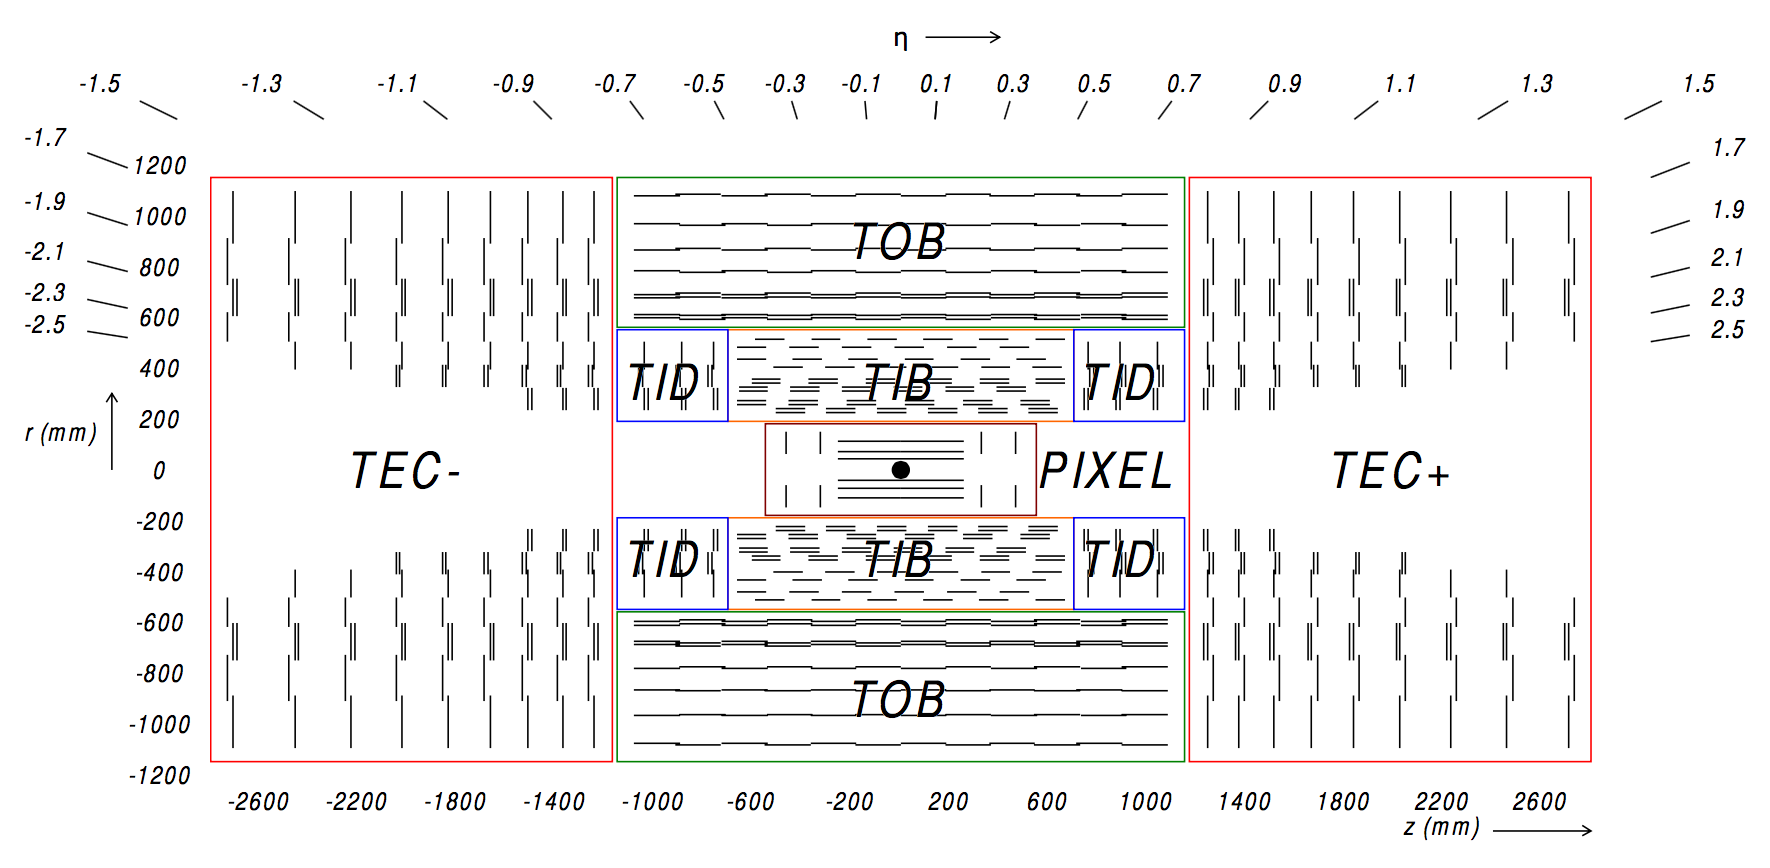
\includegraphics[width=\textwidth]{img/I-3-cms/tracker.png}
      \caption{Schematic representation of the Compact Muon Solenoid detector installed at LHC \cite{1748-0221-3-08-S08004}.}
      \label{fig:I-3-tracker}
    \end{figure}

    The barrel pixel tracker contains 768 modules for a total of 48 million pixels. The disks of the endcaps are divided into 24 segments each composed of 7 modules which yields a total number of 672 modules with 18 million pixels for the both endcaps. Each pixel is 150 $\mu$m $\times$ 100 $\mu$m in size with a thickness of 260 $\mu$m to 300 $\mu$m resulting in a single point hit resolution of 15 $\mu$m to 20 $\mu$m. \\

    The silicon strip tracker is divided into three subsystems. The Tracker Inner Barrel and Disks (TIB/TID) are composed of 4 layers in the barrel and 3 disks in each endcap, covering a region up to 55 cm. The strips are 320 $\mu$m thick and run parallel to the beam pipe in the barrel and radially in the disks. The strip pitch is of 80 $\mu$m in the two first layers of the TIB and 120 $\mu$m in the two next ones, resulting in a spatial resolution of respectivly 23 $\mu$m and 35 $\mu$m. In the TID, the pitch varies between 100 $\mu$m and 141 $\mu$m. Surroungind the TIB and TID is the Tracker Outer Barrel (TOB) composed of 6 barrel layers of 500 $\mu$m thick strips. It provides a resolution of 53 $\mu$m for the first four layers and 35 $\mu$m for the two last ones. Closing the TOB on both sides are the Tracker EndCaps (TEC) which each hold 9 disks. In addition, given modules are equipped with a second strip detector mounted back-to-back with a stereo angle of 100 mrad to provide a measurment of the second coordinate.

  \section{The Electromagnetic Calorimeter}

    The Electromagnetic Calorimeter (ECAL) of CMS is composed of lead tungstene (PbWO$_4$) crystals that act as hermetic calorimeters: they initiate the particle cascades and providing the proportionnal response to the energy deposition. The barrel counts 61 200 crystals closed by 7 324 crystals in each endcap. In order to distinguish pion shower, a high granularity preshower is installed in front of the ECAL, providing detailed measurments of the impact points. \\

    The structure of the ECAL is shown in Figure \ref{fig:I-3-ecal}. In the barrel, the ECAL covers a pseudorapidity range $ | \eta | $ < 1.479 and is divided in 360 sections in $ \phi $ and 170 in $ \eta $. The crystals cross-section varies between 22 mm $ \times $ 22 mm to 26 mm $ \times $ 26 mm for a length of 230 mm corresponding to 25.8 radiation lengths. In the endcaps, the modules cover a pseudorapidity 1.479 < $ | \eta | $ < 3.0. Each crystal has a front cross-section of 28.62 mm $ \times $ 28.62 mm and a length of 220 mm. They are grouped in units of 5 $ \times $ 5 crystals called supercrystals further inserted in one of the two \emph{Dees} that compose an endcap and maintains the ECAL in place. The preshower uses a lead radiators to initiate the avalanche that will be detected by silicon strips to measure the deposited energy and the avalanche profile. \\

    \begin{figure}[h!]
      \centering
      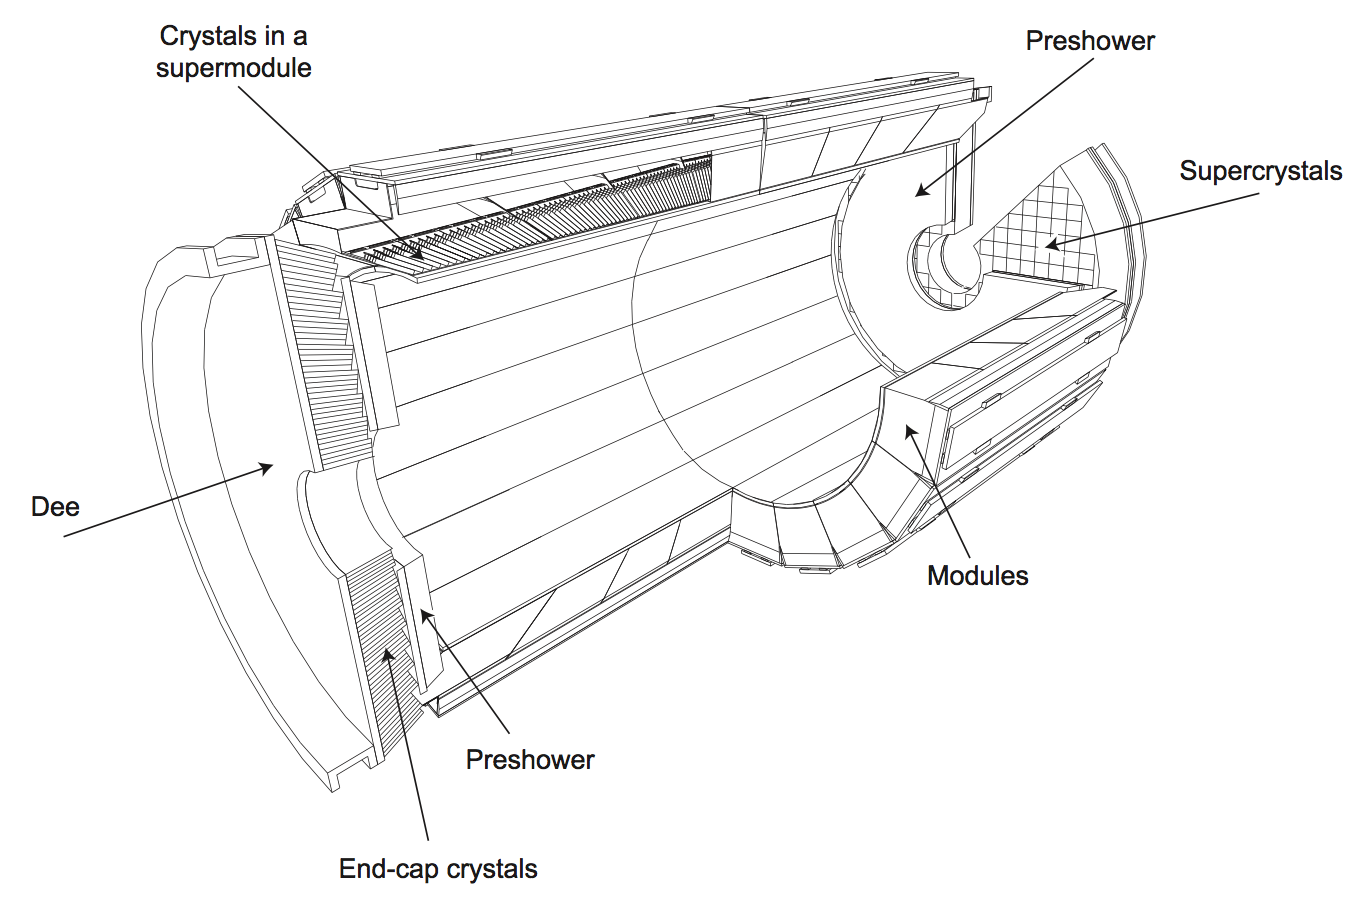
\includegraphics[width=\textwidth]{img/I-3-cms/ecal.png}
      \caption{Layout of the ECAL and disposition of the crystals in modules and supermodules \cite{1748-0221-3-08-S08004}.}
      \label{fig:I-3-ecal}
    \end{figure}

    The energy resolution of the ECAL for particles with energy bellow 500 GeV is parametrized by the following equation:
    \begin{equation}
      \left( \frac{\sigma}{E} \right)^2 = \left( \frac{S}{\sqrt{E}} \right)^2 + \left( \frac{N}{E} \right)^2 + C^2
    \end{equation}
    where $ S $ is the stochastic term, $ N $ the noise terme, and $ C $ the constant term. The main contributions to the stochastic term are relatated to fluctuations in the lateral shower containment, photostatique contributions, and fluctuations in the energy deposition inside the preshower radiators compared to what is measured by the silicon detector. The noise term includes noise from the electronics, the digitisation, and pile-up. Finally, the constant term accounts for non-uniformities in the crystals, callibration errors, and leakage of energy from the back of the crystals. From test beams, the values of $ S $, $ N $, and $ E $, where found to be so that: \\
    \begin{equation}
      \left( \frac{\sigma}{E} \right)^2 = \left( \frac{2.8\%}{\sqrt{E}} \right)^2 + \left( \frac{0.12}{E} \right)^2 + (0.30\%)^2
    \end{equation}

  \section{The Hadron Calorimeter}

    The Hadron Calorimeter (HCAL) is divided into a barrel region (HB), two endcaps regions (HE), and an outer calorimeter (HO) placed right outside the magnet as represented in Figure \ref{fig:I-3-hcal}. An additionnal forward calorimeter (HF) is place in the very forward region of CMS. The HB sits between the ECAL and the magnet at radii of 1.77 m and 2.95 m respectivly which limits the amout of material and thus absorption lengths that can be used, justifying the need for the HO to catch the trail of the cascades. \\

    \begin{figure}[h!]
      \centering
      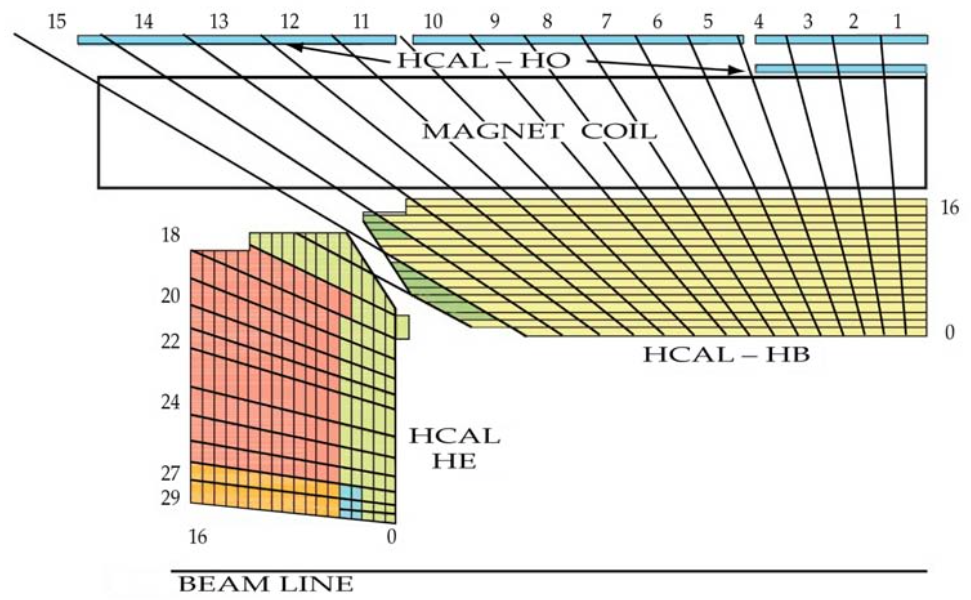
\includegraphics[width=\textwidth]{img/I-3-cms/hcal.png}
      \caption{Layout of the HCAL and disposition of the crystals in modules and supermodules \cite{1748-0221-3-08-S08004}.}
      \label{fig:I-3-hcal}
    \end{figure}

    The HB uses a sampling calorimeter design that consists of a succession of metal sheets positonned parallel to the beam that act as absorber and plastic scintillators to measure the energy deposition. The absorber is made of a 40 mm thick front steel panel, followed by eight 50.5 mm thick brass sheets, six 56.5 mm thick brass panels, and a 75 mm thick steel back plate for a total minimum of 5.82 interaction lengths. The scintillators are designed out of 3.7 mm thick Kuraray SCSN81 plastic and placed after each layer of metal. An additionnal layer of 9 mm thick Bicron BC408 is placed in front of the first steel panel in order to sample hadronic showers that might have formed in the ECAL. The HE uses 79 mm thick brass plates spaced by 9 mm gaps in which the plastic Bicron BC408 scintillators are inserted. The segmentation of the HE results in a granularity of $ \Delta \eta \times \Delta \phi $ = 0.087 $ \times $ 0.087 for $ | \eta | $ < 1.6 and 0.17 $ \times $ 0.17 for $ | \eta | $ $ \le $ 1.6. In the $ | \eta | $ < 1.3 region, hadron showers are not entierly contained in the HB and HE thus justifying the installation of the HO outside of the magnet to catch the trail of the cascades. This has a significant impact on high energy cascades and to measure the missing energy of an event, i.e. the energy carried by non-interracting particles. The HO has a minimum thickness of 1.4 interaction lengths and is segmented in 5 rings further divided into segments. Each segment has a granularity similar to the HB of 0.087 $ \times $ 0.087 in $ \Delta \eta \times \Delta \phi $. Limited by the muon system, the HO has been allocated 40 mm of space, from which 16 mm is used for the scintillators and the rest is filled with support material.

  \section{The Superconducting Magnet}

    The superconducting magnet of CMS measures 6 m of diameter for 12.5 m in length and has been design to generate a 4 T magnetic field. The return of the magnetic field lines is done through the steel yokes that support the muon chambres of CMS as represented in Figure  \ref{fig:I-3-cms-magnet} in which the amplitude of the magnetic field inside CMS has been measured using cosmic muons. The magnet is composed of four layers of winded NbTi conductor which offers very low resistance to the nominal 19.14 kA current that is required. To reach the superconducting state of the magnet, it needs to be cooled down to 1.8 K. \\

    \begin{figure}[h!]
      \centering
      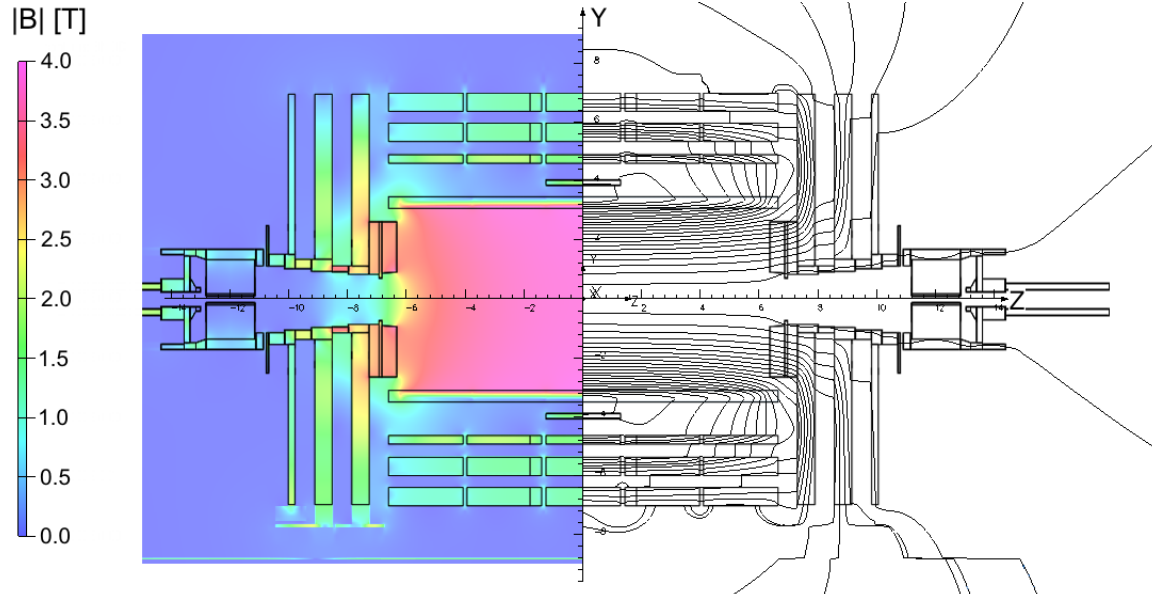
\includegraphics[width=\textwidth]{img/I-3-cms/magnet.png}
      \caption{??? \cite{Chatrchyan:2009si}.}
      \label{fig:I-3-cms-magnet}
    \end{figure}


  \newcommand{\GeVc}{GeV c$ ^{-1} $}
  \newcommand{\um}{$ \mu $m}
  \newcommand{\us}{$ \mu $s}
  \newcommand{\pT}{$ p_T $}
  \newcommand{\pZ}{$ p_Z $}
  \newcommand{\axis}[1]{#1}



  \section{The Muon System}


  			The intense magnetic field of CMS is created by cooling a solenoid down to 4.5 K, temperature at which the metal becomes supra-conductive, and by passing strong currents through it. The resulting field is uniform inside the solenoid but more complex outside, as shown in Figure \ref{fig:lhc_and_cms__cms_magnetic_field} which represents the measured magnetic field. The constant and strong field in which the tracker is placed allows it to measure the particles' transverse momentum with high-precision (resolution of less than 1\% in the tracker as seen in Figure \ref{fig:lhc_and_cms__cms_tracker_performances}). The intensity of the field is of 3.8 T inside the solenoid and typically 2 T outside the solenoid. \\

  			\begin{figure}[h!]
  				\centering
  				% 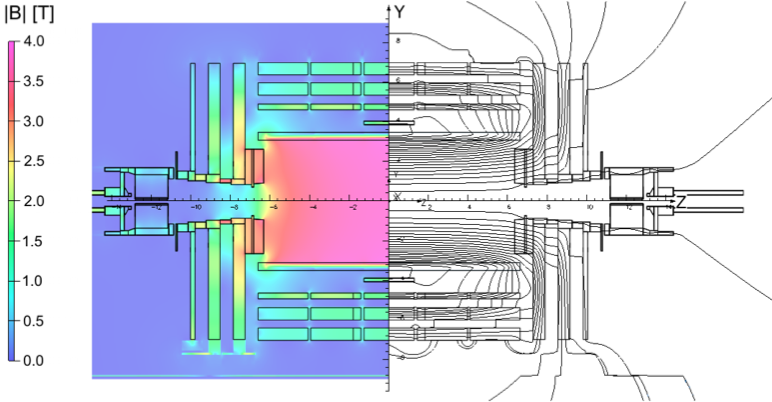
\includegraphics[width = 12cm]{2_LHC_CMS/img/cms_magnetic_field.png}
  				\caption{Field map of the magnetic field of CMS measured using cosmic rays \Cite{CMS_B_Field}.}
  				\label{fig:lhc_and_cms__cms_magnetic_field}
  			\end{figure}

  			Having the calorimeters inside the magnet improves the energy resolution as particles have less matter to travel through before reaching them, but increases the size of the solenoid. Due to the technical difficulty to build large magnets, the muon chambers are placed on the outside. This layout has the advantage to use the magnet as barrier for most particles escaping the calorimeters, ensuring that only muons will be detected by the muon system.

    \begin{figure}[h!]
      \centering
      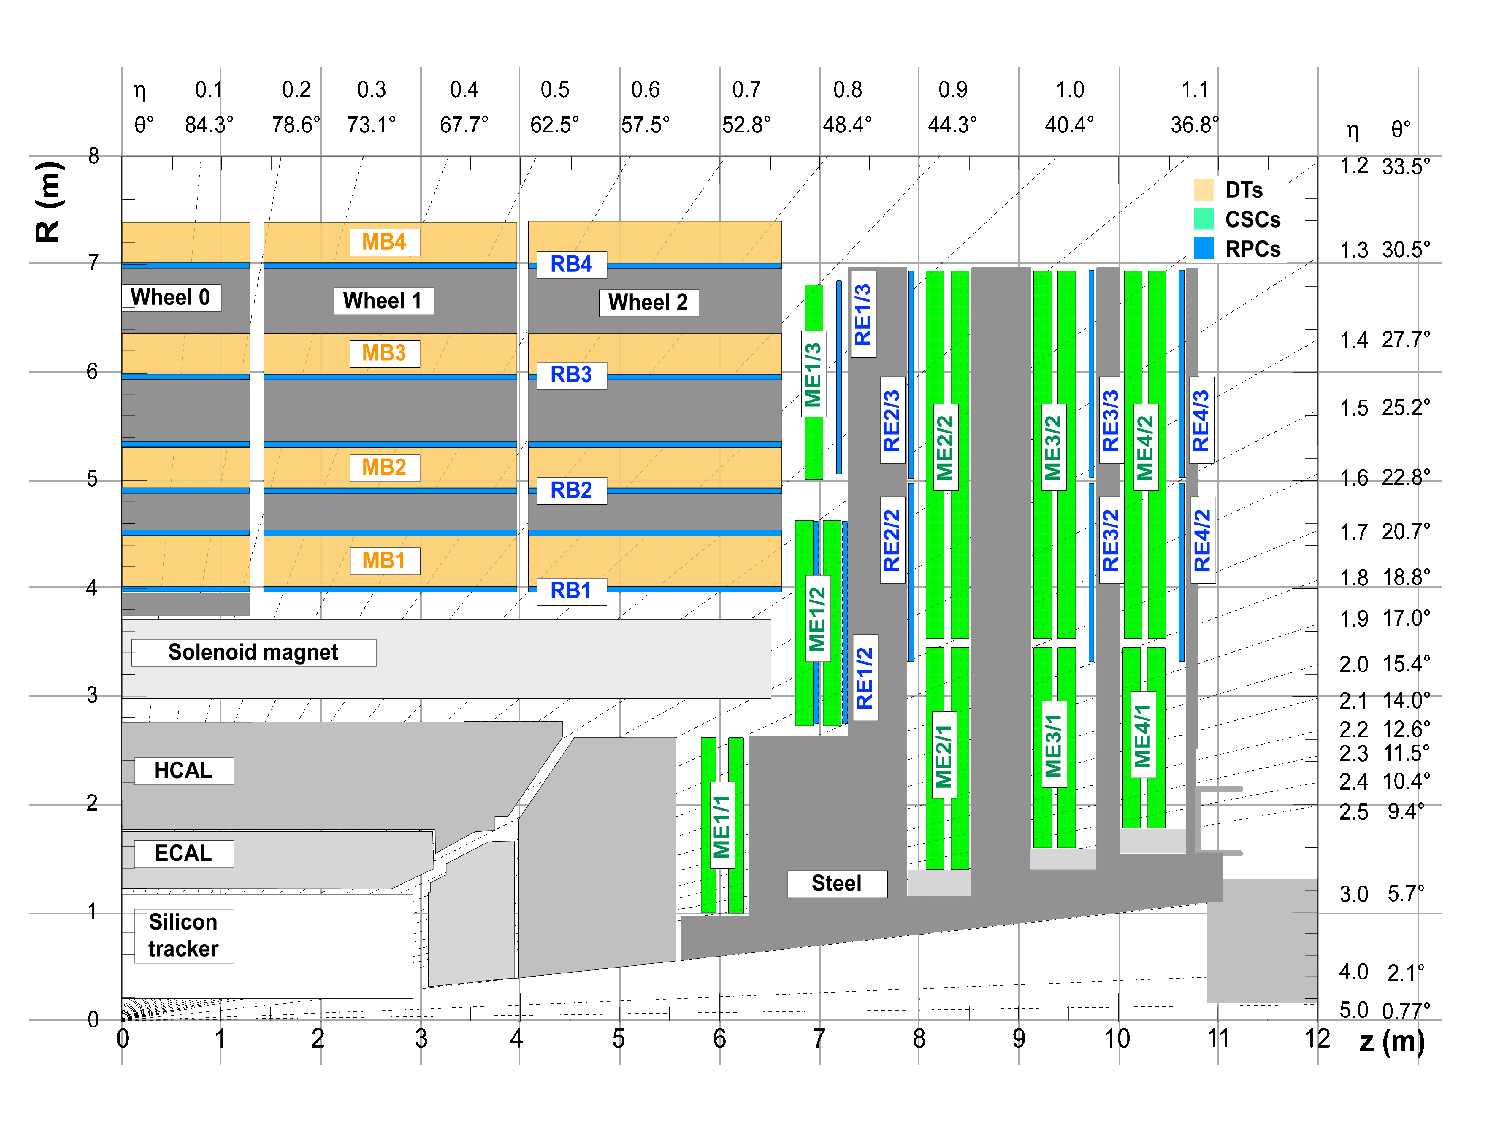
\includegraphics[width=\textwidth]{img/I-3-cms/quadrant-postls1.pdf}
      \caption{??? \cite{1748-0221-3-08-S08004}.}
      \label{fig:I-3-cms-quadrant}
    \end{figure}

    \begin{figure}[h!]
      \centering
      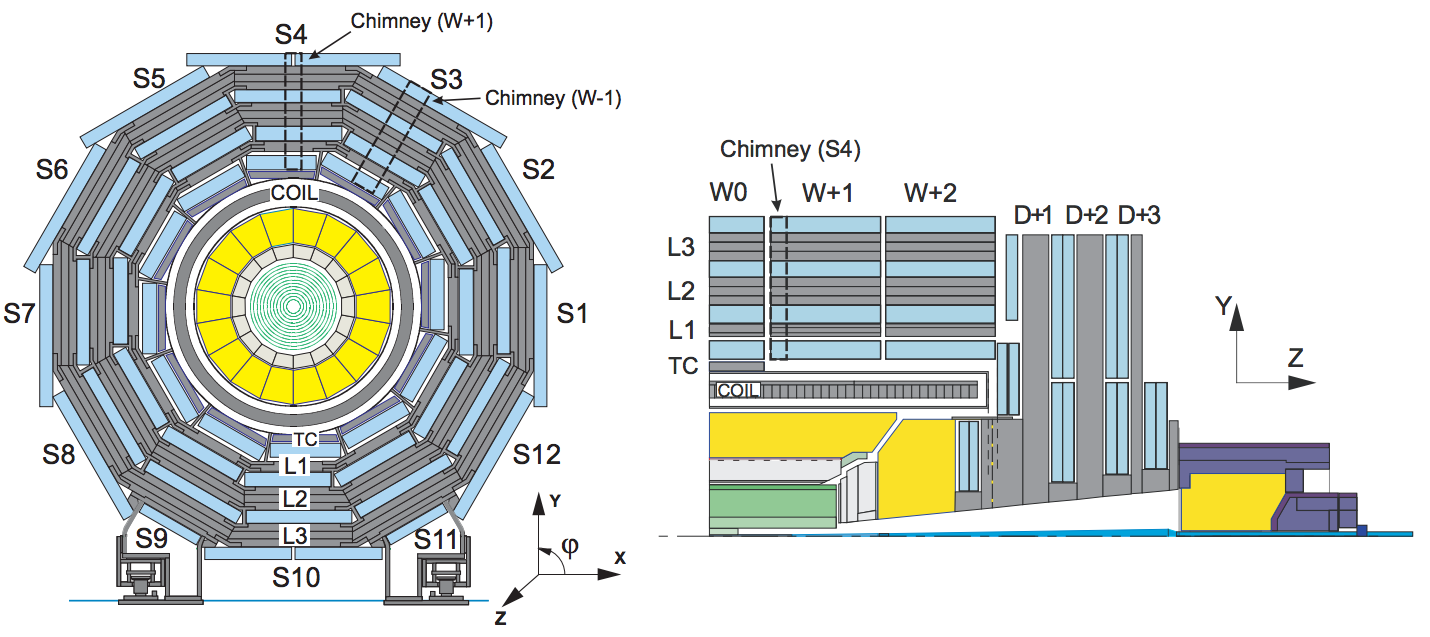
\includegraphics[width=\textwidth]{img/I-3-cms/muon-numbering.png}
      \caption{??? \cite{Chatrchyan:2009si}.}
      \label{fig:I-3-cms-muon-numbering}
    \end{figure}


    		Currently, the CMS muon system \Cite{CMS_at_LHC, CMS_Performances} is composed of three different types of gaseous detectors: \emph{Drift Tube} (DT), \emph{Cathode Strip Chamber} (CSC), and \emph{Resistive Plate Chamber} (RPC).

    		\subsection{Disposition of the Detectors}
    		\label{sec:muon_chambers__disposition_of_the_detectors}

    			Like all the CMS detectors, the muon system is divided into two regions: the barrel ($ | \eta | $ < 1) and the endcaps (1 < $ | \eta | $ < 2.4). The chambers are regrouped into stations attached to the wheels of CMS. The barrel stations contain DTs (identified by MBn) and RPCs while the endcaps stations hold CSCs (identified by MEx/y) and RPCs (identified by REn), as represented in Figure \ref{fig:muon_chambers__placement}. For financial reasons, the RPCs were not installed for the LHC's start-up in the 1.6 < $ | \eta | $ < 2.4 region where only CSCs are present.

    			\begin{figure}[h!]
    				\centering
    				% 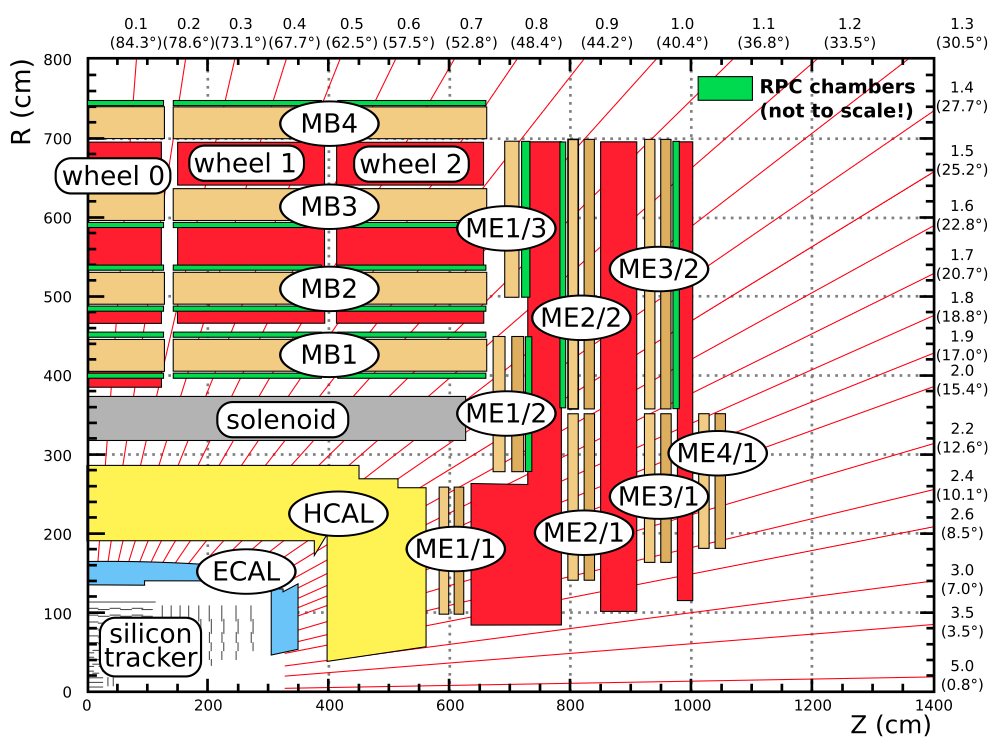
\includegraphics[width = 13cm]{3_Muon_Chambers/img/cms_chambers_placement.png}
    				\caption{Disposition of the muon chambers inside CMS. MBn refer to DTs, MEn to CSCs and the green lines to RPCs \Cite{CMS_Upgrades}.}
    				\label{fig:muon_chambers__placement}
    			\end{figure}

    			The barrel is composed of 5 wheels on which 4 layers of detectors are attached, each divided into 12 stations along $ \phi $. The endcaps have 4 layers of detectors divided into 1, 2 or 3 rings partitioned into 36 or 72 stations that overlap to ensure maximum efficiency. Figure \ref{fig:muon_chambers__cms_endcap} shows the first station of the muon endcap, ME1. The inner ring, called ME1/1 is hidden by the so-called \emph{nose}, in black. The two outer rings, ME1/2 and ME1/3 are well visible. In ME1/2, we can observe the overlap between the chambers. \\

    			\begin{figure}[p!]
    				\centering
    				% 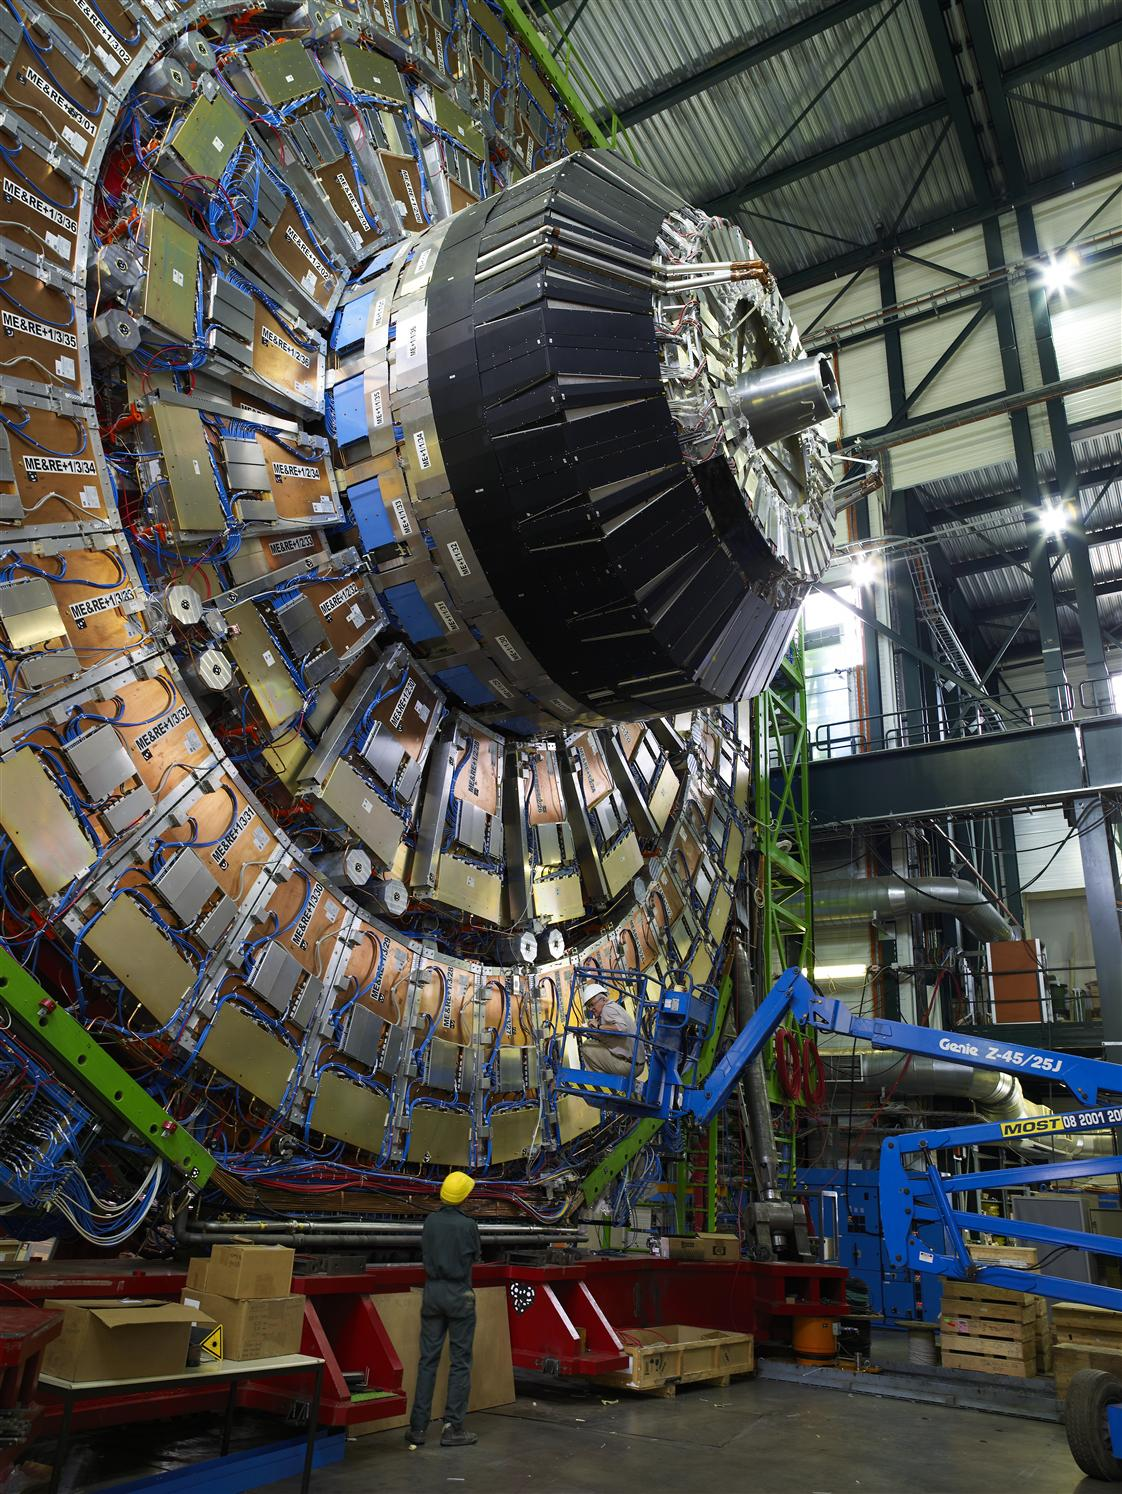
\includegraphics[width = 16.5cm]{3_Muon_Chambers/img/cms_endcap_view.jpg}
    				\caption{Picture of one of the endcaps' yokes. We can observe the two outer rings, ME1/2 and ME1/3. Chambers of the inner ring, ME1/1, are hidden inside the \emph{nose}, in black \Cite{Fig_CMS_Endcap}.}
    				\label{fig:muon_chambers__cms_endcap}
    			\end{figure}

    			The use of two different kinds of detectors in each station ensures that the system meets the required detection efficiency for muons imposed by CMS. This redundancy is crucial to select and reconstruct events with high momentum muons in the final state, signature of the Brout-Englert-Higgs boson's decay and of many processes of new physics, including super-symmetry.

    		\subsection{Drift Tubes}
    		\label{sec:muon_chambers__drift_tubes}

    			DTs are rectangular parallelepiped detectors composed of an anode wire stretched between two cathode strips as represented in Figure \ref{fig:muon_chambers__dt}. The chambers are 2.4 m long by 13 mm height by 42 mm wide. A strong electric field (of the order of 1.5 kV cm$ ^{-1} $) is formed by applying a high voltage difference between the electrodes, causing the electrons and ions to drift into the gas, and provoking avalanches near the anode. The two electrodes placed near the anode help flatten the electric field and improve the charges' drift. \\

    			\begin{figure}[h!]
    				\centering
    				% 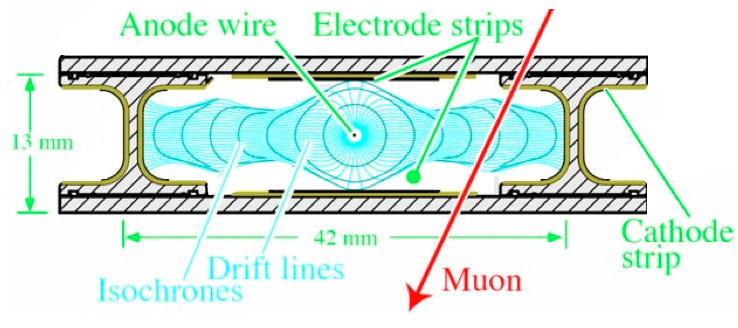
\includegraphics[width = 8cm]{3_Muon_Chambers/img/cms_dt.png}
    				\caption{Schematic view of a drift cell along with the electric field line \Cite{CMS_at_LHC}.}
    				\label{fig:muon_chambers__dt}
    			\end{figure}

    			Four DTs are assembled to create a \emph{Super Layer} (SL), and two or three SLs compose a DT module. Each SL has a spatial resolution of 100 \um{} in the direction perpendicular to the wire. To improve global precision, two SLs are used to measure the $ \phi $ coordinate and sometimes one additional SL is used to measure $ \eta $. DT modules have a time resolution of 3 ns. Their rather large size limits their rate capabilities, explaining why they are only present in the barrel where particles' fluxes are lower (< 10 Hz cm$ ^{-2} $).

    		\subsection{Cathode Strip Chambers}
    		\label{sec:muon_chambers__cathode_strip_chambers}

    			CSCs are trapezoidal multiwire proportional chambers placed in the endcaps of CMS. Multiple anode wires (about 1000 spaced by 3.2 mm) are stretched radially in the chamber above perpendicularly placed cathode strips (typically 80 separated by a pitch of 8.4 mm on the narrow side and 16 mm on the large side) as depicted in Figure \ref{fig:muon_chambers__csc}. As for the DTs, an electric field is formed between the wires and the strips, accelerating the electrons and forming the avalanches near the anodes. By reading-out both electrodes, the CSCs provide a measurement of both coordinates.

    			\begin{figure}[h!]
    				\centering
    				% 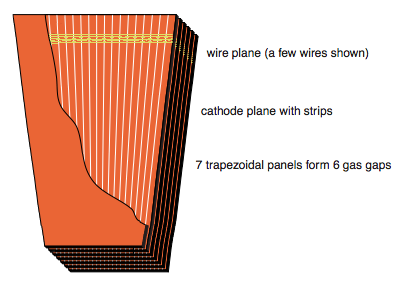
\includegraphics[height = 4.5cm]{3_Muon_Chambers/img/cms_csc.png}
    				\caption{A representation of a CSC with its wires and strips \Cite{CMS_Performances}}
    				\label{fig:muon_chambers__csc}
    			\end{figure}

    			One CSC module is made out of six chambers put together (7 cathode planes and 6 wire planes). Due to the large number of readout channels in these modules, the spatial resolution is as good as 33 \um{} for ME1/1 and ME1/2, and 80 \um{} for the other stations. The time resolution for one cathode plane is 11 ns that can be brought down to the order of 5 ns when combining the measurements of all the planes. The largest CSC modules, ME2/2 and ME3/2, are 3.4 m by 1.5 m. \\

    			Note that the two dimensional readout configuration can create ambiguities called \emph{ghosts particles} as shown in Figure \ref{fig:muon_chambers__ghosts}. When two particles hit the chamber (left), four possibilities arise when reading the output signal (right). Two of them correspond to real particles, and the two others to ghost particles. It is easy to see that for $ n $ particles interacting in the chamber, $ n^2 $ particles can be reconstructed. This limits the rates at which the CSCs can function to 1 kHz cm$ ^{-2} $.

    			\begin{figure}[h!]
    				\centering
    				% 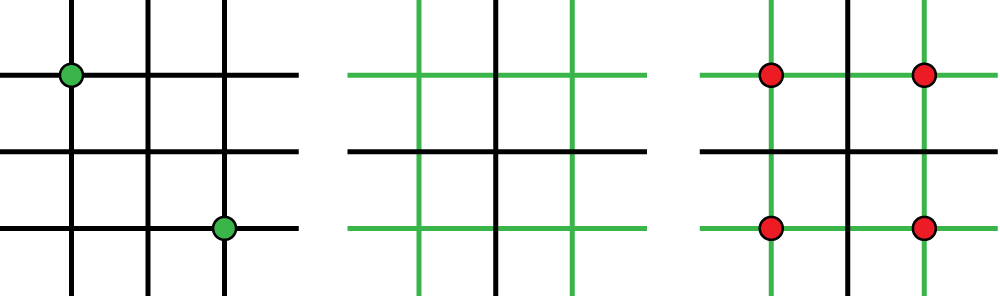
\includegraphics[width = 8cm]{3_Muon_Chambers/img/cms_csc_ghost.png}
    				\caption{Ambiguities arise when more than one particle hit the chamber at the same time.}
    				\label{fig:muon_chambers__ghosts}
    			\end{figure}

    		\subsection{Resistive Plate Chambers}
    		\label{sec:muon_chambers__resistive_plate_chambers}

    			RPCs, represented in Figure \ref{fig:muon_chambers__rpc}, are gaseous parallel plate detectors. They consist of two parallel plates, made out of bakelite with a high resistivity (10$ ^{10} $ to 10$ ^{11} $ $ \Omega $ cm) separated by a gas gap of a few millimeters. The outer surfaces of the resistive materials are coated with conductive graphite to form the HV and ground electrodes. Due to the fact that ions and electrons never come in contact with the electrodes, the evacuation time can be of importance if too many charges are produced. Therefore, the gain of the detectors are reduced and most of the amplification is done by the readout electronics and not by avalanches. This allows the RPCs to run at rates up to 1 kHz cm$ ^{-2} $, while maintaining an excellent time resolution down to 1 ns. On the other hand, they have a poor spatial resolution of the order of 1 mm. \\

    			\begin{figure}[h!]
    				\centering
    				% 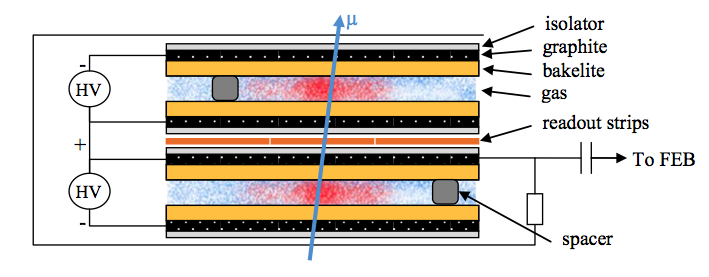
\includegraphics[width = 10cm]{3_Muon_Chambers/img/cms_rpc.png}
    				\caption{Representation of an RPC with two gas gaps for one readout strip plane \Cite{These_Karol}.}
    				\label{fig:muon_chambers__rpc}
    			\end{figure}

    			Since the RPCs can operate at high hit rate, they are used in both the barrel and the endcaps as trigger system. In the barrel, RPCs are rectangular chambers covering the DTs, while in the endcaps, they have a trapezoidal shape like the CSCs.

    		\subsection{System Performances}
    		\label{sec:muon_chambers__system_performances}

    			Figure \ref{fig:muon_chambers__performances} represents the resolution on the transverse momentum $ p_T $ of muons as a function of the pseudo-rapidity $ \eta $ for the muon system in standalone (left) and combined with the tracker's data (right). The standalone system suffers from discontinuities in $ \eta $ when transitioning from the barrel to the endcaps ($ | \eta | $ = 1) or between stations in the endcaps where particles are not detected. These imprecisions can be removed by considering data from the trackers, which also improves the overall precision by a factor of 10. For a muon with a transverse momentum of 10 \GeVc{}, the resolution goes down from about 10\% in the standalone reconstruction to about 1\% when considering the tracker.

    			\begin{figure}[h!]
    				\centering
    				% 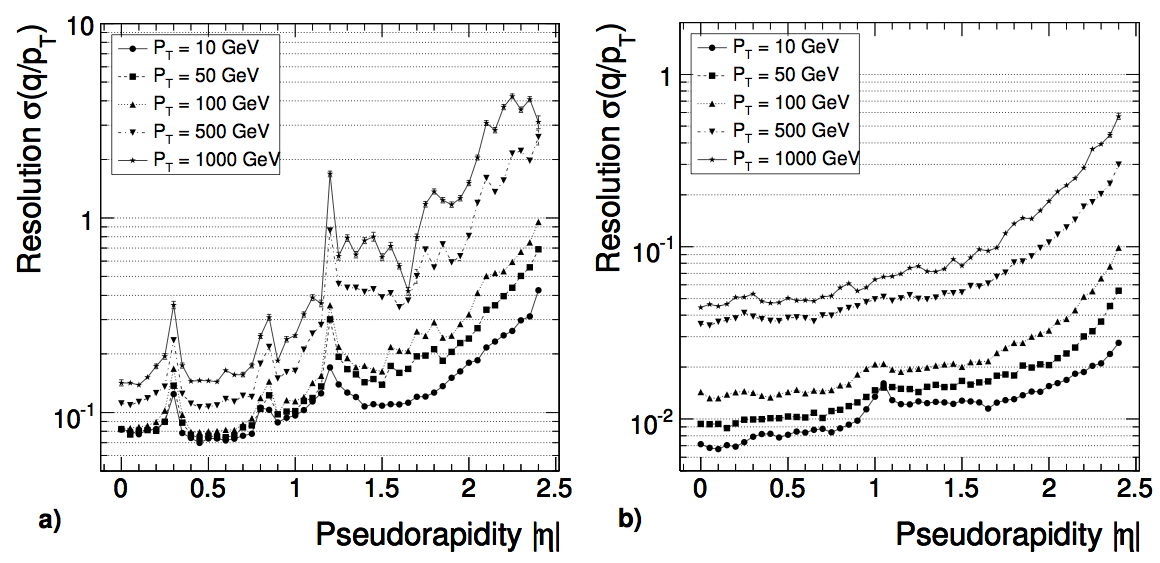
\includegraphics[width = 13cm]{3_Muon_Chambers/img/cms_muon_performances.png}
    				\caption{Resolution on the transverse momentum $ p_T $ of muons as a function of the pseudo-rapidity $ \eta $ for the muon system in standalone (left) and combined with the tracker's data (right) \Cite{CMS_Performances}.}
    				\label{fig:muon_chambers__performances}
    			\end{figure}

    \section{The Trigger System}




    		With the LHC running at a rate of 40,000,000 collisions per second, the amount of data produced by CMS is considerable ($ \sim $ 40 TB s$ ^{-1} $). We do not yet have the technology to transfer nor handle all this information. Therefore, a selection of interesting events has to be done in order to reduce the transfer's rate. The decision to keep or drop an event is taken by the CMS trigger system which includes two stages: the \emph{Level-1 Trigger} (L1 Trigger) and the \emph{High Level Trigger} (HLT) \Cite{CMS_at_LHC}. \\

    		Figure \ref{fig:trigger_system_and_reconstruction_algorithms__rates} depicts the different stages of the trigger and the maximal rate of events kept by each one of them, starting at 40 MHz and ending at 100 Hz. The kept events are sent and stored in multiple locations around the world (called \emph{Tiers}) where physicists can analyze them.

    		\begin{figure}[h!]
    			\centering
    			% 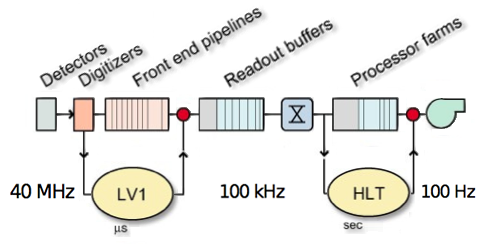
\includegraphics[width = 10cm]{5_Trigger/img/trigger_rates.png}
    			\caption{Data rates at each stage between the detectors and the data storage center. \Cite{CMS_Trigger_System}}
    			\label{fig:trigger_system_and_reconstruction_algorithms__rates}
    		\end{figure}

    		\subsection{Level-1 Trigger}
    		\label{sec:trigger_system_and_reconstruction_algorithms__level_1_trigger}

    			The L1 Trigger is the first stage of selection of CMS and has to be able to handle all events successively. Therefore, it has to take a "keep or drop" decision every 25 ns (time between two BXs). The system is composed of dedicated electronic chips for each detector placed either on CMS or in the service caverns next to it, to protect them from radiations. A diagram of the L1 Trigger's decision flow is shown in Figure \ref{fig:trigger_system_and_reconstruction_algorithms__l1}. The decision is first taken locally by small groups of muon chambers and calorimeters before being sent to the \emph{Global Muon Trigger} (GMT) \Cite{Trigger_Muon} and \emph{Global Calorimeter Trigger} (GCT) respectively, that analyze the event over all the regions. Finally, the GMT and GCT send their keep/drop signal to the \emph{Global Trigger} (GT). As represented, the tracker is not involved in this first stage selection due to the time needed to reconstruct and transfer the output data. \\

    			\begin{figure}[h!]
    				\centering
    				% 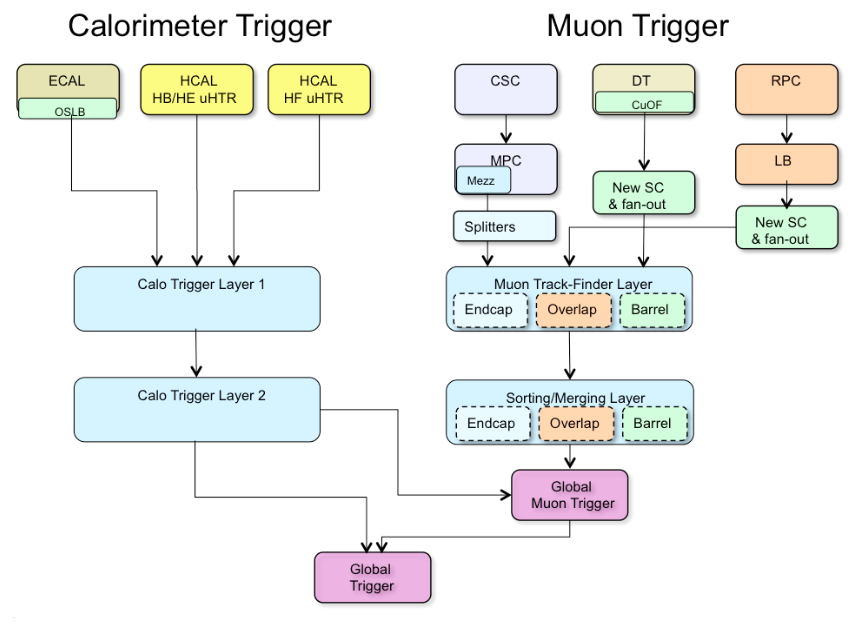
\includegraphics[width = 10cm]{5_Trigger/img/l1.png}
    				\caption{L1 Trigger decision flow of CMS before data is being transfered to the DAQ \Cite{CMS_at_LHC}.}
    				\label{fig:trigger_system_and_reconstruction_algorithms__l1}
    			\end{figure}

    			When a collision occurs, every 25 ns, the system reads out the response of every detector and stores it in a buffer that holds the last 128 events. Consequently, the algorithms have a maximum of 3.2 \us{} to process each event and return their decision. This also allows the decision taking process to be differed between the different triggers (GMT and GCT) as the particles take a certain time to travel from the IP to the various detectors. Once an algorithm has made a decision, it sends a one bit signal to the GMT or GCT. When all the detectors have responded, the GT either drops the event or tells the DAQ system to transfer it to the HLT. \\

    			% The fact that the trigger has to take a decision every 25 ns while the data is available for 3.2 \us{} motivates the use of multiple algorithms running in parallel. It is for example possible to execute 128 programs at the same time, each running for 3.2 \us{}. Every 25 ns, a different program would finish its analysis and return a keep or drop signal, allowing the overall system to respond to the L1 Trigger constraints. \\

    			As the L1 Trigger only relies on the calorimeters and on the muon system, the events' selection is done according to the signature and transverse energy left in the calorimeters, and to the transverse momentum reconstructed by the muon system. Only the transverse components of the energy and the momentum are considered as they reflect the physics of the event. Indeed, when the protons collide, the fraction of energy put at play in the interaction is not the same. Therefore, the produced particles will be boosted along \axis{Z} according to these differences, while the total transverse momentum should remain null as the collisions are head to head.

    		\subsection{High Level Trigger}
    		\label{sec:trigger_system_and_reconstruction_algorithms__high_level_trigger}

    			The HLT is composed of a farm of computers running reconstruction software that can perform complex calculations. Due to the filtering made by the L1 Trigger, the incoming data rate is lower (100 kHz), allowing for a longer processing time, of the order of 1 s. If an event passes through the multiple filters and is accepted, it is send to the storage unit and made available for analysis. Since this work aims to study track reconstruction performed at L1, the HLT will not be further reviewed.

    		\subsection{Muon System L1 Trigger}
    		\label{sec:trigger_system_and_reconstruction_algorithms__muon_system_l1_trigger}

    			The different muon chambers have their own trigger system which benefits from the detectors strengths. DTs and CSCs have excellent spatial resolution (respectively of the order of 100 and 80 \um{}) and will therefore be used to filter the events according to their transverse momentum. RPCs on the other hand have great timing capabilities (down to 1 ns) which yields good BX assignment. By combining the DTs and RPCs in the barrel, and the CSCs and RPCs in the endcaps, the GMT can reconstruct event with a multitude of muons in the final state.

    			\subsubsection{Drift Tubes and Cathode Strip Chambers}
    			\label{sec:trigger_system_and_reconstruction_algorithms__dt_and_csc}

    				DTs and CSCs use the same trigger system, the \emph{Track-Finder} (TF) \Cite{Track_Finder}, which relies on the measurement of the particles' bending angle when they pass through the detectors. The system is divided into a local and a global trigger. The local trigger validates hits in DT and CSC modules, before transmitting the information to the global trigger which tries to reconstruct tracks over all the stations.

    				\paragraph*{Local Trigger}
    				\label{sec:trigger_system_and_reconstruction_algorithms__local_trigger}

    					DT modules are divided into smaller segments as represented on the left in Figure \ref{fig:trigger_system_and_reconstruction_algorithms__dt_local}. Each couple of layers (AB, AC, AD, etc) is used to compute the position $ \mathbf{x} $ and the angle $ \phi_b $ of the track by measuring the arrival time of the signals to the anode. The further away a particle passes from the wire, the longer the drift time is, hence the time at which the signals are detected. If the values match for several couples, the segment is considered to represent a valid track and marked as such. The number of couples that return the same value defines the quality of the track. If an ambiguity appears, the parameters with the best quality are selected. \\

    					\begin{figure}[h!]
    						\centering
    						% 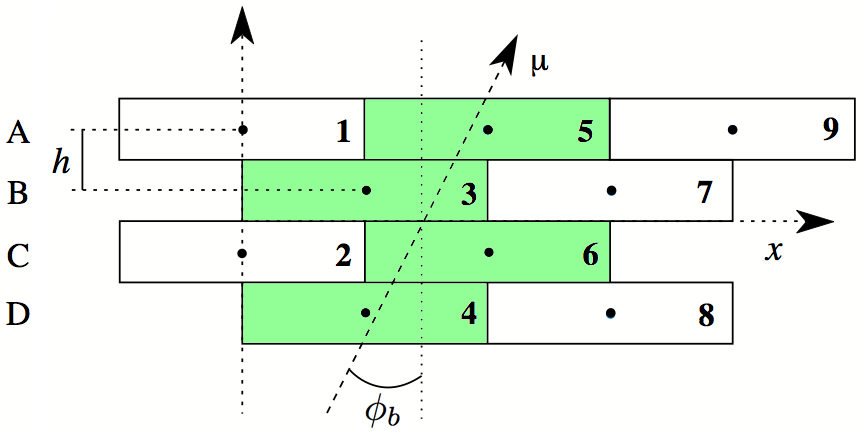
\includegraphics[height = 3.5cm]{5_Trigger/img/l1_dt_local.png}
    						% 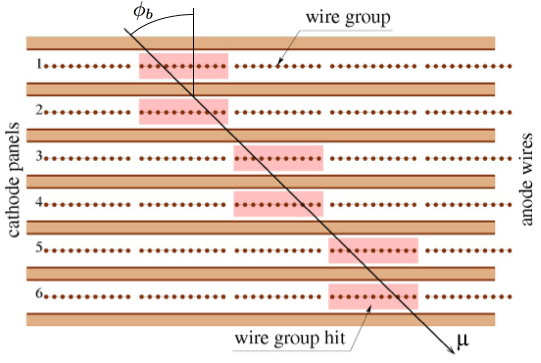
\includegraphics[height = 3.5cm]{5_Trigger/img/l1_csc_local.png}
    						\caption{DTs' local trigger measuring the particle's incident angle using the ions' drift time (left) \Cite{CMS_at_LHC}; CSCs' local trigger relying on the multiple layers to measure the particle's incident angle (right) \Cite{Trigger_Muon}.}
    						\label{fig:trigger_system_and_reconstruction_algorithms__dt_local}
    					\end{figure}

    					The same is done in CSC modules using the six planes of anode wires and seven planes of cathode strips, as seen on the right in Figure \ref{fig:trigger_system_and_reconstruction_algorithms__dt_local}. Due to the short amount of time available to run the reconstruction, anode wires are grouped by 5 to 16 by performing a logical \emph{OR} of the binary readout result.

    				\paragraph*{Global Trigger}
    				\label{sec:trigger_system_and_reconstruction_algorithms__global_trigger}

    					Once tracks have been reconstructed locally, the TF matches the different stations by comparing their hits. Figure \ref{fig:trigger_system_and_reconstruction_algorithms__dt_global} shows the pairwise matching between stations (left), the muon track (left; green), and the reconstructed track in the transverse plane (left; red). First, using the local reconstructed angle $ \phi_b $ of the track (middle), the parameters are extrapolated between layers (right) by using predefined parameters stored in LUTs for all the possible matching segments
    					\begin{equation}
    						\phi_{extrapolation} = \phi_b + \phi_{deviation} \ ,
    					\end{equation}
    					where $ \phi_{extrapolation} $ is the extrapolated parameter, and $ \phi_{deviation} $ is the deviation in $ \phi $ between two detection planes. If the extrapolation is close to the measurement, within a predefined range (right; blue), the site is added to the track and the propagation continues towards the next station. This method can result in more than one reconstructed track, which is why only the four tracks with the highest quality (best match between extrapolation and measurements, most matches, etc) are kept. Finally, an estimation of the transverse momentum in function of the bending angle is done.

    					\begin{figure}[h!]
    						\centering
    						% 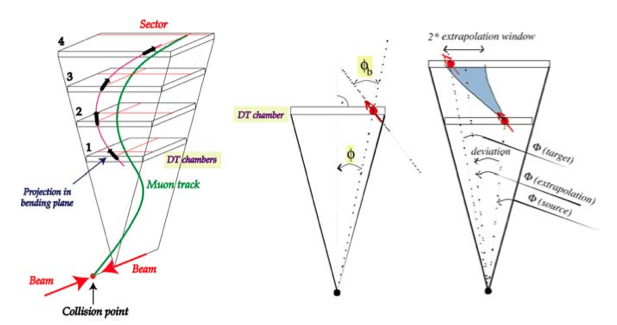
\includegraphics[width = 12cm]{5_Trigger/img/l1_track_finder.png}
    						\caption{Reconstructed trajectory by the Track-Finder using pairwise matching between the stations \Cite{CMS_at_LHC}.}
    						\label{fig:trigger_system_and_reconstruction_algorithms__dt_global}
    					\end{figure}

    			\subsubsection{Resistive Plate Chambers}
    			\label{sec:trigger_system_and_reconstruction_algorithms__rpc_l1_trigger}

    				RPCs use a \emph{Pattern Comparator} (PAC) algorithm \Cite{These_Karol} to retrieve the transverse momentum of the tracks. Each station is divided into segments that are considered to be active if they have been hit, or inactive otherwise. The state of the segments is read out by multiple chips that try to match the hits against a list of preloaded patterns they hold in a LUT. In order to fill the LUT, simulations are ran for a finite number of transverse momenta $ p_T $, associating a code, $ p_T^{Code} $, and a numerous amount of possible patterns to each one of them. For each $ p_T^{Code} $, a ranking is done according to the importance of the patterns
    				\begin{equation}
    					E(pattern, \; p_T^{Code}) = \frac{N_0(pattern, \; p_T^{Code})}{N(p_T^{Code})} \ ,
    				\end{equation}
    				where $ N_0 $ is the number of identical patterns given by the same $ p_T^{Code} $, and $ N $ is the total number of patterns given by the $ p_T^{Code} $. Patterns are added to the LUT, starting with those with the highest $ E $, until 90 to 95\% of the tracks for each $ p_T^{Code} $ are present. \\

    				\begin{figure}[h!]
    					\centering
    					% 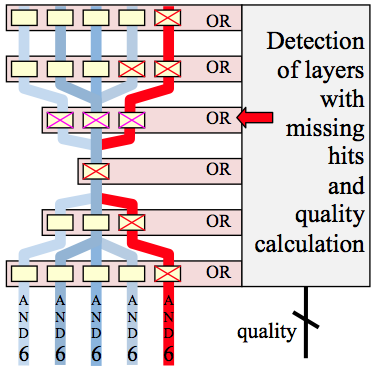
\includegraphics[width = 6cm]{5_Trigger/img/l1_rpc.png}
    					\caption{Pattern Comparator (PAC) algorithm matching hits against a multitude of predefined patterns \Cite{These_Karol}.}
    					\label{fig:trigger_system_and_reconstruction_algorithms__rpc}
    				\end{figure}

    				Figure \ref{fig:trigger_system_and_reconstruction_algorithms__rpc} shows a couple of patterns that are being tested against measurements. If a layer has not been hit, all the segments are set to active, but the quality of the resulting track will be degraded. The four best reconstructed tracks in the barrel and the endcaps are kept and sent to the GMT.

    			\subsubsection{Global Muon Trigger}
    			\label{sec:trigger_system_and_reconstruction_algorithms__global_muon_trigger}

    				For each event, the GMT receives the four best matches from the TF and from the PAC for the barrel and the endcaps. Those are compared and the best candidates are combined to increase the precision.

    			\subsubsection{System Performances}
    			\label{sec:trigger_system_and_reconstruction_algorithms__system_performances}

    				An important parameter of the L1 Trigger is the applied threshold or cut on the transverse momentum above which all events are accepted. Figure \ref{fig:trigger_system_and_reconstruction_algorithms__acceptance} shows the generated (produced inside CMS; black line) and accepted (reconstructed and accepted by the L1 Trigger; red dots) rate of events according to the applied cut on the transverse momentum $ p_{T; threshold} $ for events with a single muon in the final state. Ideally, the dotted curves should match the continuous line, meaning that the system is able to perfectly identify the muons. Unfortunately, numerous low energy muons are reconstructed with a much higher energy, misleading the trigger. Improving those results would lead to a lower cut as the rates at high energies would drop. The current threshold is at 14 \GeVc{} (blue arrow) which yields a rate of the order of 2 kHz. The selection on a single muon is only one among several tens of L1 Trigger filters. The total bandwidth of the L1 Trigger has to be shared between all the muons, the electrons, the photons, and the jets triggers. Therefore, the maximum event rate allowed to the single muon trigger is limited to 2 kHz. \\

    				\begin{figure}[h!]
    					\centering
    					% 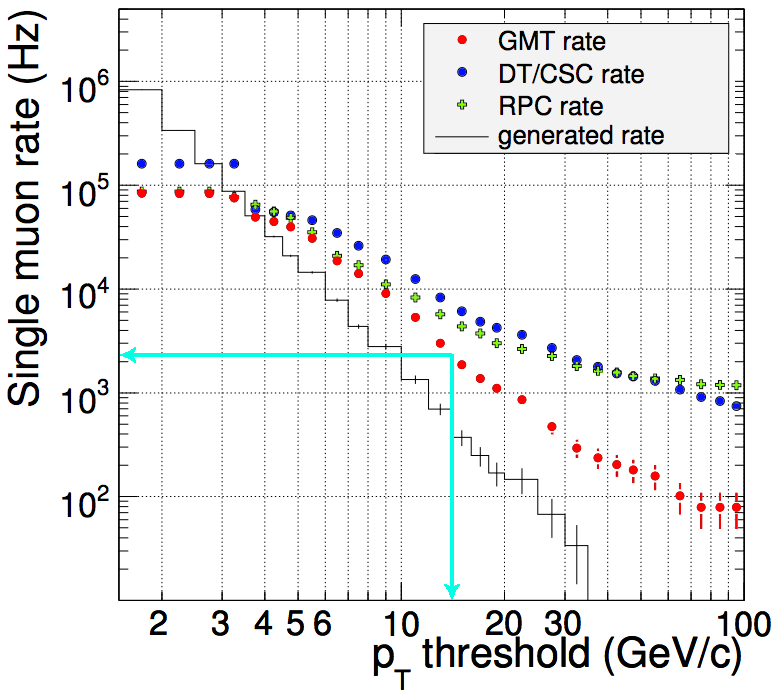
\includegraphics[width = 8cm]{5_Trigger/img/l1_acceptance.png}
    					\caption{Generated and accepted rate of events for the L1 Trigger according to their transverse momentum $ p_T $ \Cite{CMS_Performances}.}
    					\label{fig:trigger_system_and_reconstruction_algorithms__acceptance}
    				\end{figure}

    				Figure \ref{fig:trigger_system_and_reconstruction_algorithms__l1_cut} presents the L1 Trigger's efficiency as a function of the transverse momentum $ p_T $ (left) and pseudo-rapidity $ \eta $ (right) for a single muon. The plot on the left is called a \emph{turn-on} plot and shows the acceptance for various $ p_T $ for a defined threshold (14 \GeVc{}). Ideally, the curves should be equal to 0 below the cut and to 1 above the cut. Instead, because of the finite transverse momentum resolution in the muon track reconstruction, the trigger starts to accept events already above 5 \GeVc{}, and only keeps around 95 \% of them above the threshold. The second plot emphasizes what has been reviewed in Section \ref{sec:muon_chambers__ls2_upgrade_and_challenges}, namely the fact that efficiency drops at high $ | \eta | $ due to the lack of redundancy in the muon system.

    				\begin{figure}[h!]
    					\centering
    					% 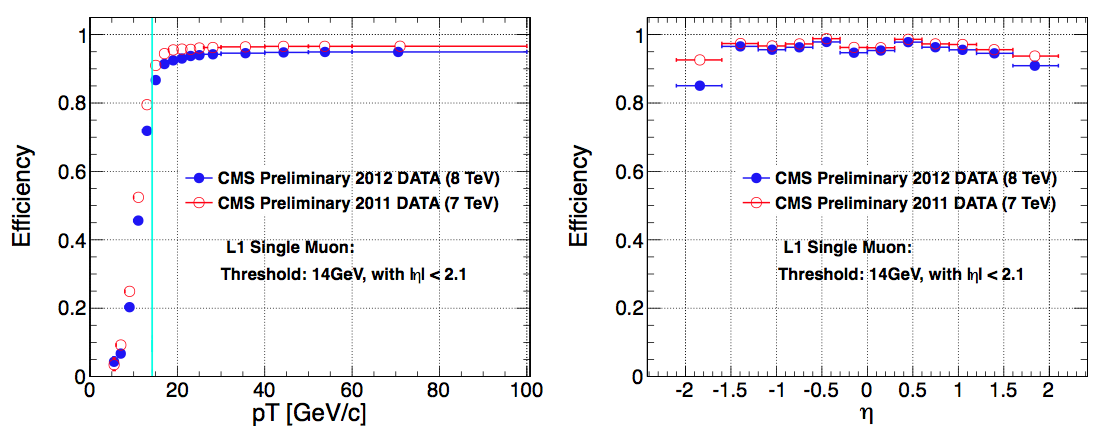
\includegraphics[width = 12cm]{5_Trigger/img/l1_efficiency.png}
    					\caption{L1 Trigger's reconstruction efficiency as a function of the transverse momentum $ p_T $ (left) and pseudo-rapidity $ \eta $ (right) of single muons \Cite{CMS_L1_Efficiency}.}
    					\label{fig:trigger_system_and_reconstruction_algorithms__l1_cut}
    				\end{figure}
